\section{Theory}
\label{sec:theory}

This section collects what can be said about the equilibria of a trained model before any computation. Classical degree
theory fixes their bookkeeping: a bounded model has an odd number of equilibria, every additional pair contains an
unstable one, and the index sum certifies whether a numerically found set is complete (Theorem~\ref{thm:degree}). It
does not fix how many pairs there are; that is set by training. Proposition~\ref{prop:forced} identifies when reproducing
the true equilibria forces additional, spurious ones, and Proposition~\ref{prop:manifold} shows that an attractor of the
model is excited from an equilibrium through the unstable manifold of that equilibrium (Fig.~\ref{fig:schematic}). Proofs are
given in Appendix~\ref{app:proofs}.

\begin{figure*}
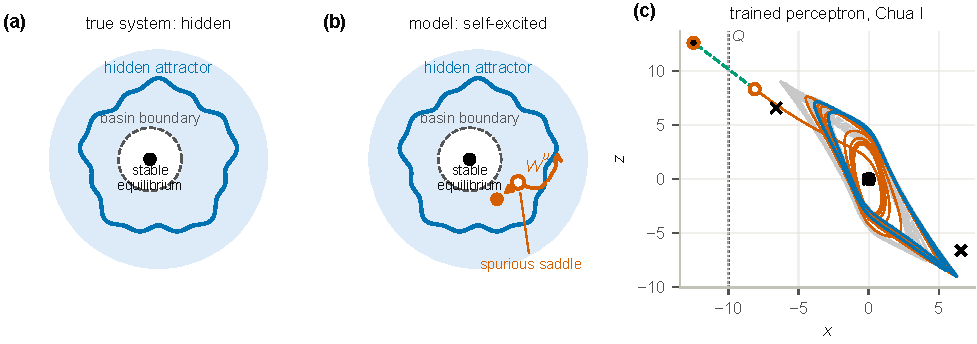
\includegraphics[width=\textwidth]{figures/fig_schematic.pdf}
\caption{How a model loses hiddenness. (a) In the true system the basin of the hidden attractor (shaded) is separated from
the stable equilibrium by a basin boundary, so no trajectory started near the equilibrium reaches the attractor. (b) A
trained model reproduces the attractor but has an additional pair of equilibria; one branch of the unstable manifold $W^u$
of the spurious saddle lands on the attractor, which is therefore excited from the saddle (Proposition~\ref{prop:manifold}).
(c) A real case: a one-layer perceptron with $32$ hidden units trained on Chua's circuit in regime~I (training set HE1),
projected on the $(x,z)$ plane. Gray: the hidden attractor of the true system; blue: the attractor reproduced by the model;
crosses: true equilibria. The model copies the stable origin (black circle) and has two spurious equilibria, a saddle (open
circle) $2.3$ units away from the nearest true saddle-focus, possibly its displaced continuation, and a stable equilibrium
outside the region $Q$ (filled, orange edge; dotted line: the boundary $x=-10$ of $Q$).
One branch of the saddle's unstable manifold (dashed) ends on the spurious stable equilibrium; the other (solid, first $450$
steps) winds onto the reproduced attractor, which is therefore self-excited in the model. Of $20$ such perceptrons trained
with different seeds, $18$ reproduce a hidden attractor, and in $8$ of them a branch of a spurious saddle lands on it.}
\label{fig:schematic}
\end{figure*}

\subsection{Index sum of a bounded map}
\label{sec:degree}

Let $F:\mathbb{R}^N\to\mathbb{R}^N$ be the model map of Sec.~\ref{sec:models}. A fixed point $r^*=F(r^*)$ is
\emph{nondegenerate} if $F$ is differentiable at $r^*$ and $\det\bigl(I-DF(r^*)\bigr)\neq0$; its index is
\begin{equation}
\ind(r^*)=\operatorname{sign}\det\bigl(I-DF(r^*)\bigr).
\label{eq:index}
\end{equation}
For the echo state network with activation $\phi$, $DF(r^*)=\operatorname{diag}\bigl(\phi'(Ar^*+b)\bigr)A$; for hard-tanh activation the diagonal
holds zeros and ones (saturated and linear neurons).

\begin{theorem}[Index sum]
\label{thm:degree}
Let $F$ be continuous with bounded image, $\|F(r)\|_\infty\le R$ for all $r$. Then for every $c>R$ the topological
degree of $\mathrm{id}-F$ on the cube $(-c,c)^N$ with respect to $0$ equals~$1$. If all fixed points of $F$ are
nondegenerate, there are finitely many of them and
\begin{equation}
\sum_{r^*=F(r^*)}\ind(r^*)=1.
\label{eq:indexsum}
\end{equation}
\end{theorem}

This is the Lefschetz--Hopf theorem for a map of a cube into its interior;\cite{GranasDugundji2003Fixed,Deimling1985NFA}
we state it because it applies to every bounded model, whatever the training. For the echo state network $R=1$; for a
perceptron with a bounded output layer $R$ is set by its last weights and bias. The cube is taken strictly larger than the
image because fixed points can lie on its boundary, as they do for hard-tanh networks with saturated neurons. If $F$ only
maps a compact convex set $K$ into its interior, the indices of the fixed points in $K$ sum to $1$, which covers
dissipative models with unbounded output. The index has a direct dynamical reading.\cite{KatokHasselblatt1995Intro}

\begin{lemma}
\label{lem:parity}
For a nondegenerate fixed point, $\ind(r^*)=(-1)^\ell$, where $\ell$ is the number of real eigenvalues of $DF(r^*)$ greater
than~$1$, counted with algebraic multiplicity.
\end{lemma}

\begin{corollary}
\label{cor:counts}
Let all $K$ fixed points of $F$ be nondegenerate and let $U$ be the number of unstable ones. Then
(i) $K$ is odd;
(ii) exactly $(K-1)/2$ fixed points have index $-1$, each of them is unstable, and hence $U\ge(K-1)/2$;
(iii) if a numerically found set $\hat E$ of fixed points has $\sum_{\hat E}\ind\neq1$, then $\hat E$ is incomplete.
\end{corollary}

Item (ii) means that every additional pair of equilibria brings at least one unstable equilibrium, and item (iii) gives a
check of root finding that costs nothing once the Jacobians are known; the converse fails, since a missed pair of indices
$+1$ and $-1$ leaves the sum unchanged. Index sums of this kind constrain the fixed points of threshold-linear networks in
continuous time,\cite{Curto2019TLN,Morrison2024TLN} and degree arguments prove that unstable fixed points exist in
continuous Hopfield networks.\cite{Beise2026UnstableHopfield} For random networks the number of equilibria grows
exponentially with $N$.\cite{WainribTouboul2013,BenArous2021Counting} Theorem~\ref{thm:degree} applies to every closed-loop
echo state network and to every perceptron with a bounded output layer. It does not apply to residual networks,
$F(u)=u+g(u)$ with bounded $g$, nor to next-generation reservoir computers, whose trajectories can escape to infinity.

\subsection{Forced spurious equilibria}
\label{sec:forced}

The true system has its own equilibria, and a good model should have copies of them. Let $\varphi_h$ be the flow map of
the true system over the sampling time $h$ and $x_1,\dots,x_m$ its hyperbolic equilibria in the region $Q$. Let $\ell_j$ be
the number of real positive eigenvalues of the Jacobian $Df(x_j)$ of the vector field, counted with algebraic multiplicity,
and
\begin{equation}
\iota_j=\operatorname{sign}\det\bigl(I-D\varphi_h(x_j)\bigr)=(-1)^{\ell_j},\qquad s=\sum_{j=1}^m\iota_j.
\label{eq:trueindex}
\end{equation}
The second equality is the relation between the index of an equilibrium and that of the translation operator along the
flow:\cite{KrasnoselskiiTranslation1968} since $D\varphi_h(x_j)=\exp\bigl(h\,Df(x_j)\bigr)$, a real eigenvalue $\lambda$
contributes a factor $1-e^{h\lambda}$ of the sign of $-\lambda$, and a complex pair contributes $|1-e^{h\lambda}|^2>0$.

\begin{proposition}[Forced spurious equilibria]
\label{prop:forced}
Let $F$ be continuous with bounded image and all fixed points nondegenerate, and let $r_1,\dots,r_m$ be fixed points with
$\ind_F(r_j)=\iota_j$. Then the remaining fixed points of $F$ have total index $1-s$; if $s\neq1$, there are at least $|1-s|$
of them. The condition $\ind_F(r_j)=\iota_j$ holds if near $r_j$ there is a $C^1$ invariant manifold on which $F$ is
$C^1$-conjugate to $\varphi_h$ near $x_j$ and the block of $DF(r_j)$ transversal to it has no real eigenvalue greater
than~$1$.
\end{proposition}

Since $\iota_j=\operatorname{sign}\det\bigl(-Df(x_j)\bigr)$, $s$ is the degree of $-f$ on any ball that contains exactly
$x_1,\dots,x_m$; if $f$ points into such a ball on its boundary, this degree is $1$ by the Poincar\'e--Hopf theorem. Hence
$s\neq1$ excludes a trapping ball around the equilibria, and a bounded model of such a system must ``close'' the escaping
directions inside its bounded state space. Two cases in this study have $s\neq1$. Chua's circuit in regime~I
(Table~\ref{tab:systems}) has three equilibria with indices $(-1,-1,+1)$, so $s=-1$: a bounded model with copies of all
three needs at least two more, of total index $+2$. The Li--Sprott system used by R\"ohm \textit{et al.}\cite{Rohm2021} has
no equilibria, $s=0$, so every bounded model of it has at least one. The forced equilibria have positive total index and
may well be stable; Proposition~\ref{prop:forced} forces equilibria, not unstable ones. In the other regimes $s=1$ and
spurious equilibria are not forced: their number is set by training. Unbounded models such as residual networks escape
the constraint, whereas architectures that guarantee bounded or dissipative learned
dynamics\cite{Kaptanoglu2021Trapping,Li2022Dissipative,Linot2023Stabilized,Tang2026Dissipative} fall under it.

\subsection{Excitation through unstable manifolds}
\label{sec:manifold}

Hiddenness is decided near the equilibria. Let $\mathcal{A}$ be an attractor with basin
$B=\{x:\operatorname{dist}(F^nx,\mathcal{A})\to0\}$, and let $e\notin\mathcal{A}$ be a hyperbolic fixed point near which $F$
is $C^1$ with $DF(e)$ invertible. Its unstable manifold $W^u(e)$ is the set of points with a backward orbit
$y_0=y$, $F(y_{-n-1})=y_{-n}$, converging to $e$, and the local unstable manifold $W^u_{\mathrm{loc}}(e)$ is the part whose
backward orbit stays in a small neighborhood of $e$. For a tanh echo state network with invertible $A$, $F$ is a
diffeomorphism onto $(-1,1)^N$ and backward orbits are unique.

\begin{proposition}[Excitation criterion]
\label{prop:manifold}
(i) If $W^u(e)\cap B\neq\varnothing$, then $B$ intersects every neighborhood of $e$, i.e., $\mathcal{A}$ is excited
from~$e$. (ii) If $W^u_{\mathrm{loc}}(e)\setminus\{e\}$ does not meet the closure $\bar B$, then some neighborhood of $e$
does not intersect $B$.
\end{proposition}

\begin{corollary}
\label{cor:criterion}
$\mathcal{A}$ is excited from $e$ if and only if $W^u_{\mathrm{loc}}(e)\setminus\{e\}$ meets $\bar B$. In particular, if
$W^u(e)\setminus\{e\}$ does not meet the basin boundary, $\mathcal{A}$ is excited from $e$ if and only if
$W^u(e)\cap B\neq\varnothing$. An exciting equilibrium lies on the basin boundary $\partial B$, since $e\in\bar B$ while its
orbit stays at $e\notin\mathcal{A}$. An asymptotically stable equilibrium never excites an attractor. If all equilibria satisfy the hypotheses above and none lies
in $\mathcal{A}$, the attractor is hidden if and only if no local unstable manifold of an unstable equilibrium
meets~$\bar B$.
\end{corollary}

Part (i) is the reasoning behind the standard procedure of starting trajectories on an unstable manifold to locate
self-excited attractors;\cite{LeonovKuznetsov2013,Dudkowski2016} Corollary~\ref{cor:criterion} states when this test is also
complete. The basin boundary matters: a branch of $W^u(e)$ that crosses a codimension-one basin boundary, for instance the
stable manifold of a boundary saddle, does so robustly, and then both adjacent basins are excited. For hard-tanh networks
with saturated neurons, $DF(e)$ is singular, but $F$ is affine near a fixed point inside a linear region, and
part (ii) holds with the same proof. A practical consequence for high-dimensional models is that, to leading order in the
radius, points of a small ball around $e$ leave along $W^u(e)$ and only their projection on the unstable subspace
$E^u(e)$ matters, so the excitation test can sample directions in $E^u(e)$, of dimension $\dim W^u(e)$, instead of a ball
in $\mathbb{R}^N$ (Sec.~\ref{sec:protocol}).

\subsection{A survival heuristic}
\label{sec:heuristic}

Theorem~\ref{thm:degree} and training together supply unstable equilibria, and by Corollary~\ref{cor:criterion} each of them
destroys hiddenness as soon as its unstable manifold reaches the basin. If each of $U$ equilibria had $\nu$ branches
landing independently in $B$ with probability $p_B$, the probability that the attractor stays hidden would be
\begin{equation}
\Pr(\mathcal{A}\ \text{hidden}\mid U)\approx(1-p_B)^{\nu U},
\label{eq:heuristic}
\end{equation}
with $\nu=2$ for a one-dimensional unstable manifold with a positive eigenvalue ($\nu=1$ if the eigenvalue is below $-1$,
since the map then swaps the two branches) and $p_B$ the fraction of the region occupied by the basin. For
higher-dimensional unstable manifolds $\nu$ is only an effective parameter. Equation~\eqref{eq:heuristic} is a reference curve, not a law:
branches of different equilibria of the same model need not be independent, and where they go depends on the data the
model was trained on. Section~\ref{sec:results} measures the actual dependence on $U$ and compares it with
Eq.~\eqref{eq:heuristic}.
